%!TEX root = ./main.tex

\chapter{Approach\label{chapter:approach}}

\section{Methodology\label{section:methodology}}

To achieve this goal of enhancing the reporting functionalities of FACT
with knowledge about the past stability and popularity characteristics,
the following three steps are planned for extending FACT 
as illustrated in figure \ref{fig:FACT}.

\begin{figure}[ht]
\centering 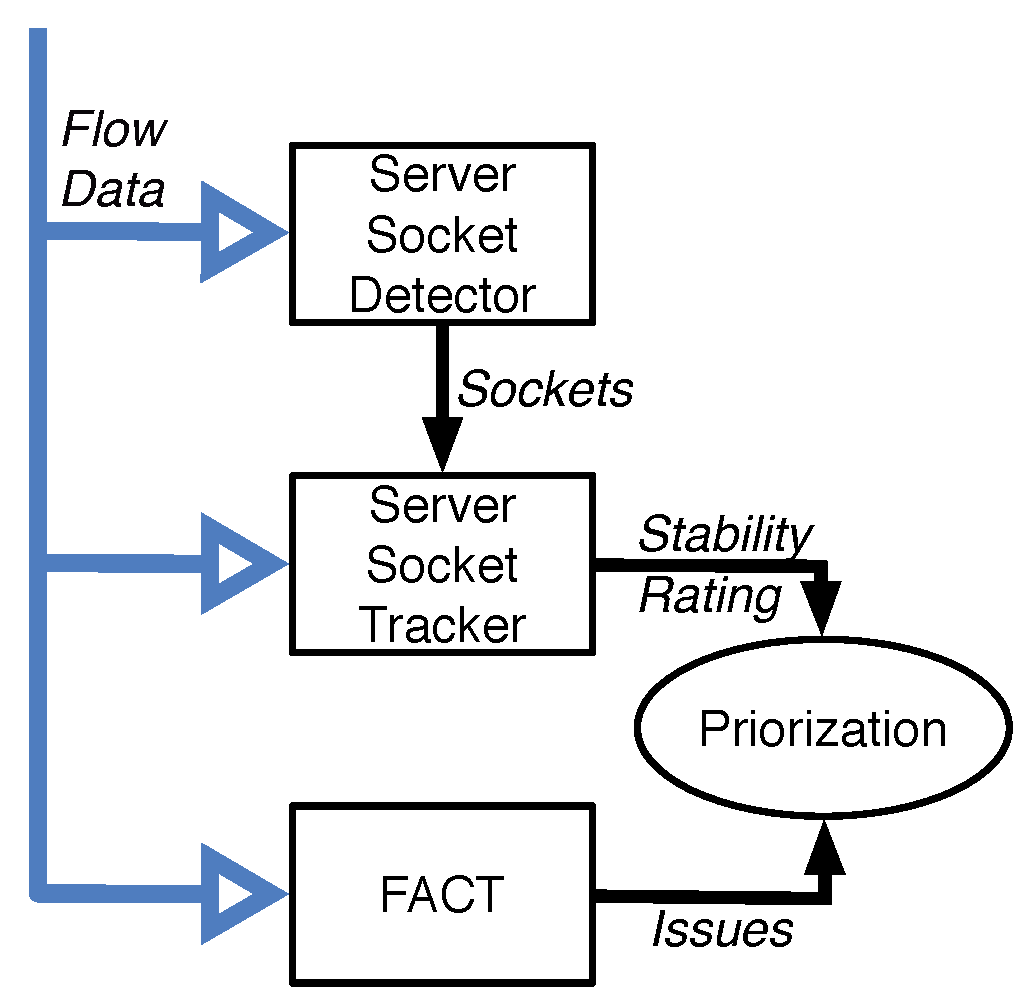
\includegraphics[width=8.5cm]{images/Approach_blockdiagram.eps}
\caption{Interactions of new components with FACT}
\label{fig:FACT}
\end{figure}

In a first step, a server socket detector is implemented. The
challenge of the server socket detection lies in the fact that the
netflow data does not provide enough precise timing information to
determine which flow is originated from the client and thus determine
the server's socket. Therefore, the server socket detection is
achieved by the assumption that server sockets act as concentrators
in the sense that several clients have connections to the identical
server socket and bases on the work shown in \cite{Schatzmann:Dissection,Schatzmann:Mining,Schatzmann:Tracing} and is discussed in more detail in section \ref{section:socket_detection}.

Secondly, the previously detected server sockets are continually
monitored and especially the successful and unsuccessful connection
attempts are recorded by the server socket tracker. 
Furthermore, these information are used to update the statistical 
information of visibility, popularity and stability. Section \ref{section:socket_tracking} covers this step in detail.

In a third step, the number of server sockets have to be reduced and
selected such that FACT is able to use these sockets
for outage tracking. In particular, the server sockets coverage of the
Internet address space has to be optimized. It makes no sense to select
only the most popular sockets if they are all located in the same /24
network.

Finally, FACT has to be adopted to optimally use the preselected and rated 
server sockets for prioritizing relevant connectivity issues by reducing 
outage alerts based on single host outages of unstable services.

%%%%%%%%%%%%%%%%%%%%%%%%%%%%%%%%%%%%%%%%%%%%%%%%%%%%%%%%%%%%%%%%%%%%%%%%%%%%%%%%
\section{Data\label{section:data}}
% briefly describe the Switch network and its topology..
% traffic volume and netflow data unsampled!

% see tech report 338 for numbers and layout?! evtl actual numbers (2012)




%%%%%%%%%%%%%%%%%%%%%%%%%%%%%%%%%%%%%%%%%%%%%%%%%%%%%%%%%%%%%%%%%%%%%%%%%%%%%%%%
\section{Flowbox\label{section:flowbox}}

\subsection{Preprocessing}
% configured with internal prefixes, responsible for tagging flows with direction. Setting transit and internal network traffic (in-in) as invalid (filtering away)

\subsection{Connection Cache}
This module is responsible for generating bidirectional flows from the incoming unidirectional flows. This is done by storing the flows in hash table with a hash key which is identical for incoming and outgoing flows. For correct operation of the biflow cache, a properly configured InOutFilter is required in front of the biflow cache since it requires that all flows must be tagged either as outgoing or as incoming. 

\subsection{Noise Cancellation}
\subsubsection{Fan-Out Filter}
% scanning detection and elimination
% state algorithm.. analog to tech report
\subsubsection{Noise Filter}
% remove single packet flows / unidirectional biflows...

\subsection{Detection of Server Sockets}
\subsubsection{Server Socket Detector}

\subsubsection{Server Socket Registry}

\subsection{Monitoring of Server Sockets}
\subsubsection{Server Socket Stability Tracker}
\subsubsection{Server Socket Selector}

\subsection{Connectivity Issue Detection}

